\documentclass[10pt,a4paper]{article}

\usepackage[utf8]{inputenc}
\usepackage[spanish]{babel}
\usepackage{graphicx}
\usepackage{fancyhdr}
\usepackage{multicol}
\usepackage[skip=6pt]{caption}
\usepackage[hidelinks]{hyperref}

\title{Interpretación remota de partituras sobre instrumentos de viento}
\author{Víctor Manuel Fernández Castro}
\date{Abril de 2016}

\setlength{\parskip}{6pt}
\fancyhead[L]{Víctor M. Fdez. Castro}
\renewcommand{\footrulewidth}{0.4pt}
\setlength{\headheight}{13.07225pt} 

% ------------------------------------------------------------------------------

\begin{document}
	
	% Portada ------------------------------------------------------------------
	
	\maketitle
	\thispagestyle{empty}
	
	% Índice -------------------------------------------------------------------
	
	\newpage
	\tableofcontents
	
	% Capítulo 1 ---------------------------------------------------------------
	
	\newpage
	\pagestyle{fancy}
	\section{Introducción y objetivos}
	
	Nuestro proyecto parte de la atención en numerosas iglesias de Granada, que
	incorporan órganos de tubos, instrumentos muy complejos, muchos de ellos
	formando parte del inmobiliario, y merecedores de un gran reconocimiento por
	la artesanía y la calidad de su construcción.
	
	Lamentablemente, muchos de ellos se encuentran en un estado de abandono, lo
	que acelera su deterioro, no se reparan y, por ello, no se pueden tocar,
	cayendo en un círculo vicioso.
	
	Además, creemos interesante la idea de que se pueda hacer sonar un órgano
	aunque no haya organista, dando la posibilidad tanto de acompañar
	celebraciones litúrgicas como de tener música de fondo durante el horario de
	visitas.
	
	\subsection{Objetivos}
	
	Nuestro propósito es ingeniar un sistema capaz de \textbf{interpretar
	partituras musicales en un órgano} suplantando las pulsaciones del artista,
	lo que incluye los siguientes objetivos:
	
	\begin{enumerate}
		\item Analizar la \textbf{mecánica real} de un órgano eclesiástico.
		
		\begin{enumerate}
			\item Tomar \textbf{medidas completas} de cada uno de los teclados,
			los pedales y las palancas de registros.
			\item \textbf{Diseñar en 3D} los componentes principales del
			instrumento.
			\item Determinar la \textbf{presión} necesaria para mover cada
			tecla, cada pedal y cada palanca del órgano.
		\end{enumerate}
		
		\item Estudiar la comunicación entre el \textit{software} y el
		\textit{hardware}, incluyendo todos los \textbf{componentes
		electrónicos} que habrá de incluir.
		
		\item Plantear distintas \textbf{alternativas de sistemas empotrados}
		que sirvan de soporte de programación.
		
		\item Analizar el \textbf{protocolo MIDI} como formato de archivo para
		almacenar partituras.
		
		\item \textbf{Diseñar} el sistema \textit{software} que cubrirá varias
		vías de comunicación entre el usuario y la mecánica, lo que comprende:
		
		\begin{enumerate}
			\item Un \textbf{servicio en segundo plano}, que atienda:
			
			\begin{enumerate}
				\item Reproducción de archivos MIDI.
				\item Comunicación inter-proceso.
				\item Receptor de un mando a distancia.
				\item Menú de control sobre el hardware, con un ''modo
				Ingeniería''.
			\end{enumerate}
			
			\item Una \textbf{aplicación \textit{web}} para controlar el
			sistema, con soporte para:
			
			\begin{enumerate}
				\item Reproducir partituras electrónicas.
				\item Instalar nuevas piezas y gestionar listas de reproducción.
				\item Configurar el mando a distancia.
			\end{enumerate}
			
			\item Una \textbf{base de datos} como soporte de almacenamiento
			persistente.
			\item Un \textbf{protocolo de comunicación} entre la aplicación
			y el servicio.
		\end{enumerate}
		
		\item \textbf{Implementar} el sistema diseñado, como:
		
		\begin{enumerate}
			\item Un demonio para Linux.
			\item Un servicio \textit{web} sobre Apache y PHP.
			\item Una base de datos MySQL.
		\end{enumerate}
		
		\item \textbf{Validar} junto al \textit{hardware} el proyecto
		desarrollado.
	\end{enumerate}
	
	El diseño del sistema electrónico, que requiere competencias de Ingeniería
	Electrónica e Industrial, fue objeto del proyecto de D. Mikel Aguayo
	Fernández.
	
	% Capítulo 2 ---------------------------------------------------------------
	
	\section{Requisitos técnicos}
	
	Para especificar el diseño de este proyecto hemos propuesto una serie de
	requisitos tanto \textit{hardware} como \textit{software}, que enumeramos a
	continuación.
	
	\subsection{Requisitos hardware}
	
	\begin{enumerate}
	
		\item Un juego de mecanismos accionará las \textbf{teclas}, otro moverá
		los \textbf{pedales} y otro desplazará los \textbf{registros} de
		timbres.
		
		\item El sistema no podrá acceder a la mecánica interna del instrumento,
		ni modificarlo de ninguna forma.
		
		\item No podrá apoyarse demasiado peso sobre el órgano, ni hacerse
		contra-apoyo (hacia arriba).
		
		\item El \textbf{control principal}, la instalación de partituras y la
		configuración se harán \textbf{remotamente}.
		
		\item Se proveerá un \textbf{control local reducido} de los accionadores
		con fines de puesta en marcha y mantenimiento.
		
		\item Asimismo se facilitará el control remoto desde un \textbf{mando a
		distancia}.
		
		\item El diseño debe ser \textbf{flexible y extensible} para distintos
		órganos.
		
		\item Se debe de poder instalar y desinstalar fácilmente.
		
	\end{enumerate}
	
	\subsection{Requisitos software}
	
	\begin{enumerate}
		
		\item Se ofrecerá \textbf{control remoto} para todos los casos de uso a
		nivel de usuario.
		
		\item La interfaz permitirá controlar la \textbf{reproducción}: iniciar
		una pieza, pausarla, reanudarla y detenerla. La reproducción por defecto
		será en modo bucle.
		
		\item Facilitará la subida y \textbf{gestión de partituras}. En dicho
		gestor se mostrará la duración de cada pieza.
		
		\item Los archivos a procesar son de formato \textbf{MIDI estándar}, sin
		perjuicio de que una partitura pueda estar adaptada específicamente al
		sistema.
		
		\item Las piezas musicales se clasificarán en \textbf{listas de
		reproducción}.
		
		\item La interfaz de usuario permitirá \textbf{asignar} dichas listas a
		ciertos botones del mando arriba mencionado.
		
		\item El \textbf{mando} tendrá capacidad para reproducir una serie de
		listas programadas, así como pausar y detener la reproducción.
		
		\item El \textit{software} dará soporte al \textbf{testeo} de los
		accionadores de forma local.
		
		\item El controlador debe ser \textbf{extensible} para órganos con más o
		menos teclas, distinto número de teclados o diferente configuración de
		registros.
		
		\item La aplicación para el usuario debe ser lo más \textbf{sencilla e
		intuitiva} posible.
		
		\item Se busca obtener una aplicación de control
		\textbf{multiplataforma}.
		
		\item La interfaz de usuario se presentará en varios \textbf{idiomas}.
		
		\item Ya que el control es remoto, se hará hincapié en la
		\textbf{seguridad}, tanto autentificación de acceso como aspectos de
		programación, tales como inyección de código.
		
	\end{enumerate}
	
	% Capítulo 3 ---------------------------------------------------------------
	
	\section{Análisis del sistema}

	Como paso previo al diseño del sistema, deberemos conocer con detalle todos
	los elementos con los que va a interactuar nuestro sistema, así como
	plantear diferentes alternativas de cara al desarrollo del
	\textit{software}.

	\subsection{Órgano de la Parroquia de Santa Fe}

	El instrumento instalado en la Parroquia de la Encarnación de Santa Fe es en
	realidad un doble órgano artesanal construido en dos fases: En 1775 se
	instaló el primer órgano, de estilo \textbf{barroco}, obra del organero
	Pedro Ghys. Posteriormente, a principios de la década de 1830, el francés
	Guillermo D'Enoyer lo amplía añadiendo un órgano \textbf{romántico}, con un
	segundo teclado y nuevos sonidos, pero todo el mecanismo es independiente
	del primer instrumento.
	
	\begin{multicols}{2}
		\noindent
		\begin{center}
			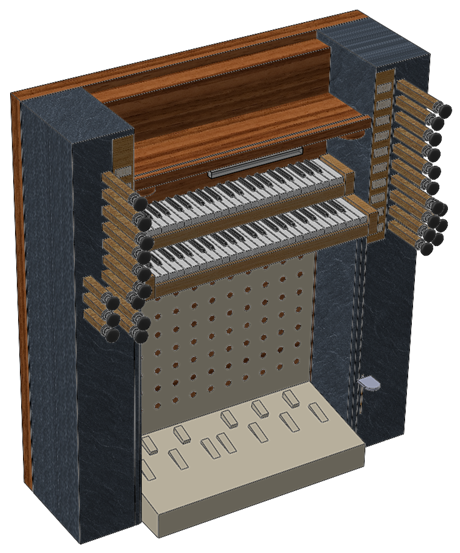
\includegraphics[width=0.4\textwidth]{images/organo} 
			\captionof{figure}{Reproducción 3D del órgano.}
		\end{center}
		\columnbreak
		Para funcionar, el órgano se alimenta de \textbf{aire}. Antiguamente se utilizaba un fuelle gigante, situado en la antesala, que llevaba el aire a una cámara de almacenamiento, para proporcionar un flujo de entrada constante. Esto requería que hubiese alguien accionándolo mientras el organista tocaba. Hoy día el fuelle ha sido sustituido por una \textbf{bomba eléctrica}.
		
		La primera tarea que llevamos a cabo fue conocer el órgano en profundidad, tomar algunas medidas y \textbf{diseñar el modelo en 3D} con el \textit{software} \textit{SolidWorks}.
	\end{multicols}
	
	\begin{multicols}{2}
		\noindent
		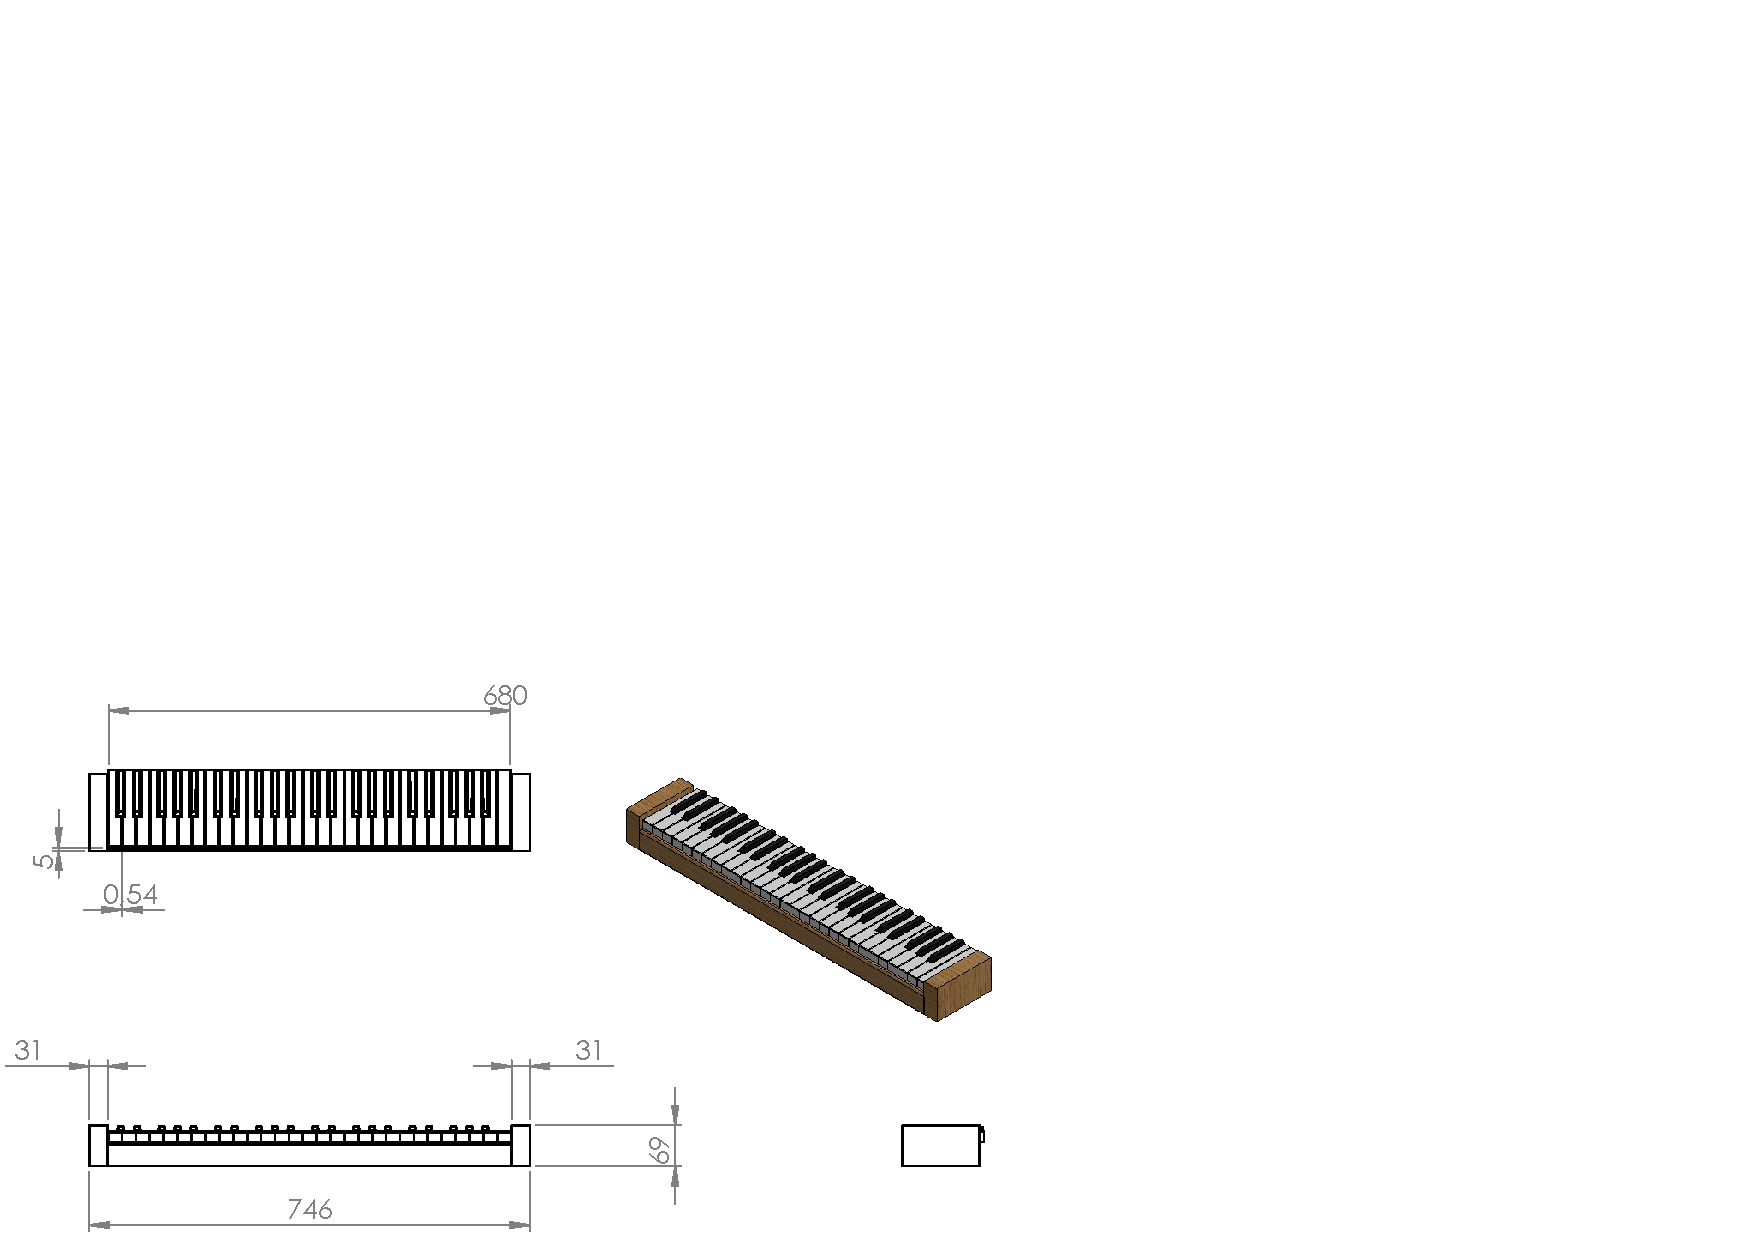
\includegraphics[width=0.5\textwidth]{images/teclado_modelo} 
		\captionof{figure}{Medidas del teclado.}
		\columnbreak
		Tenemos dos teclados de cuatro octavas notas cada uno, el de arriba, correspondiente al órgano barroco, y otro más abajo, que sobresale del primero, para el órgano romántico, de la misma extensión.
	\end{multicols}
	
	\begin{multicols}{2}
		\noindent
		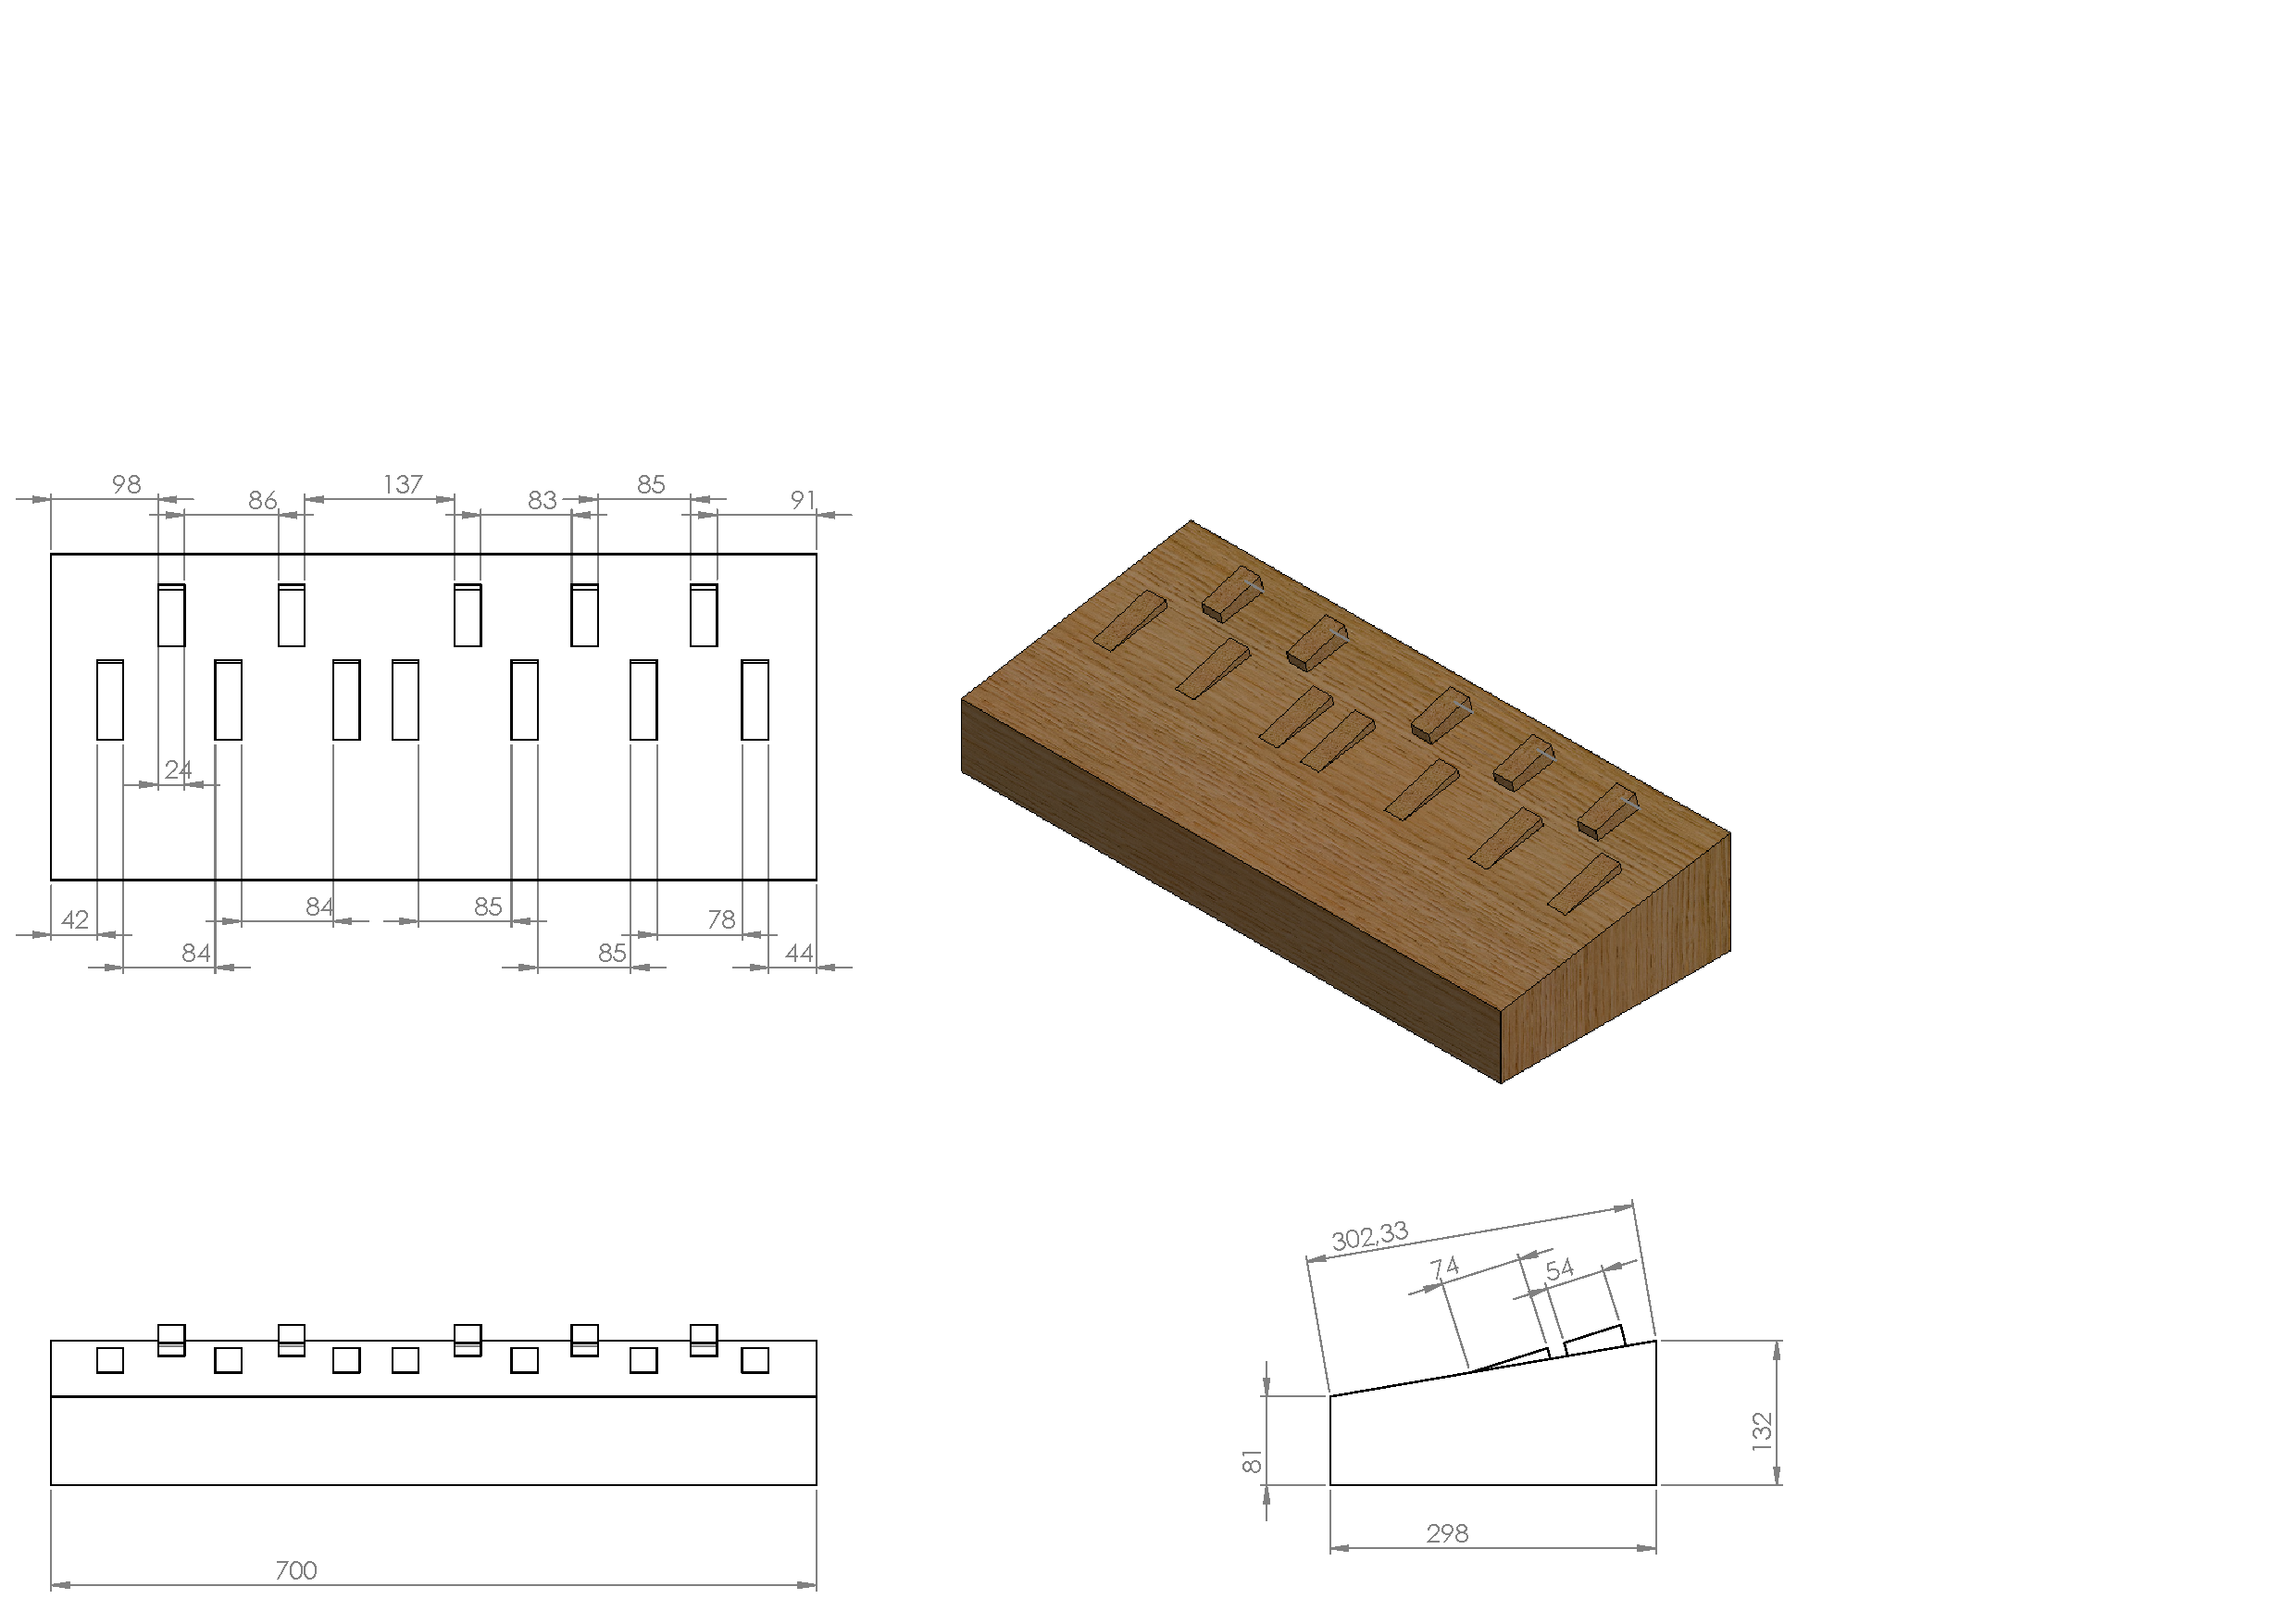
\includegraphics[width=0.5\textwidth]{images/pedalier_modelo} 
		\captionof{figure}{Medidas del pedalier.}
		\columnbreak
		Este órgano cuenta con un \textit{pedalier} con un registro fijo: el \textbf{bajo de \textit{contrast}}. Los pedales están dispuestos en forma de escala diatónica, igual que las teclas. Cada pedal tiene aproximadamente la misma anchura que una tecla aunque, obviamente, están más separados unos de otros.
	\end{multicols}
	
	\begin{multicols}{2}
		\noindent
		\begin{center}
			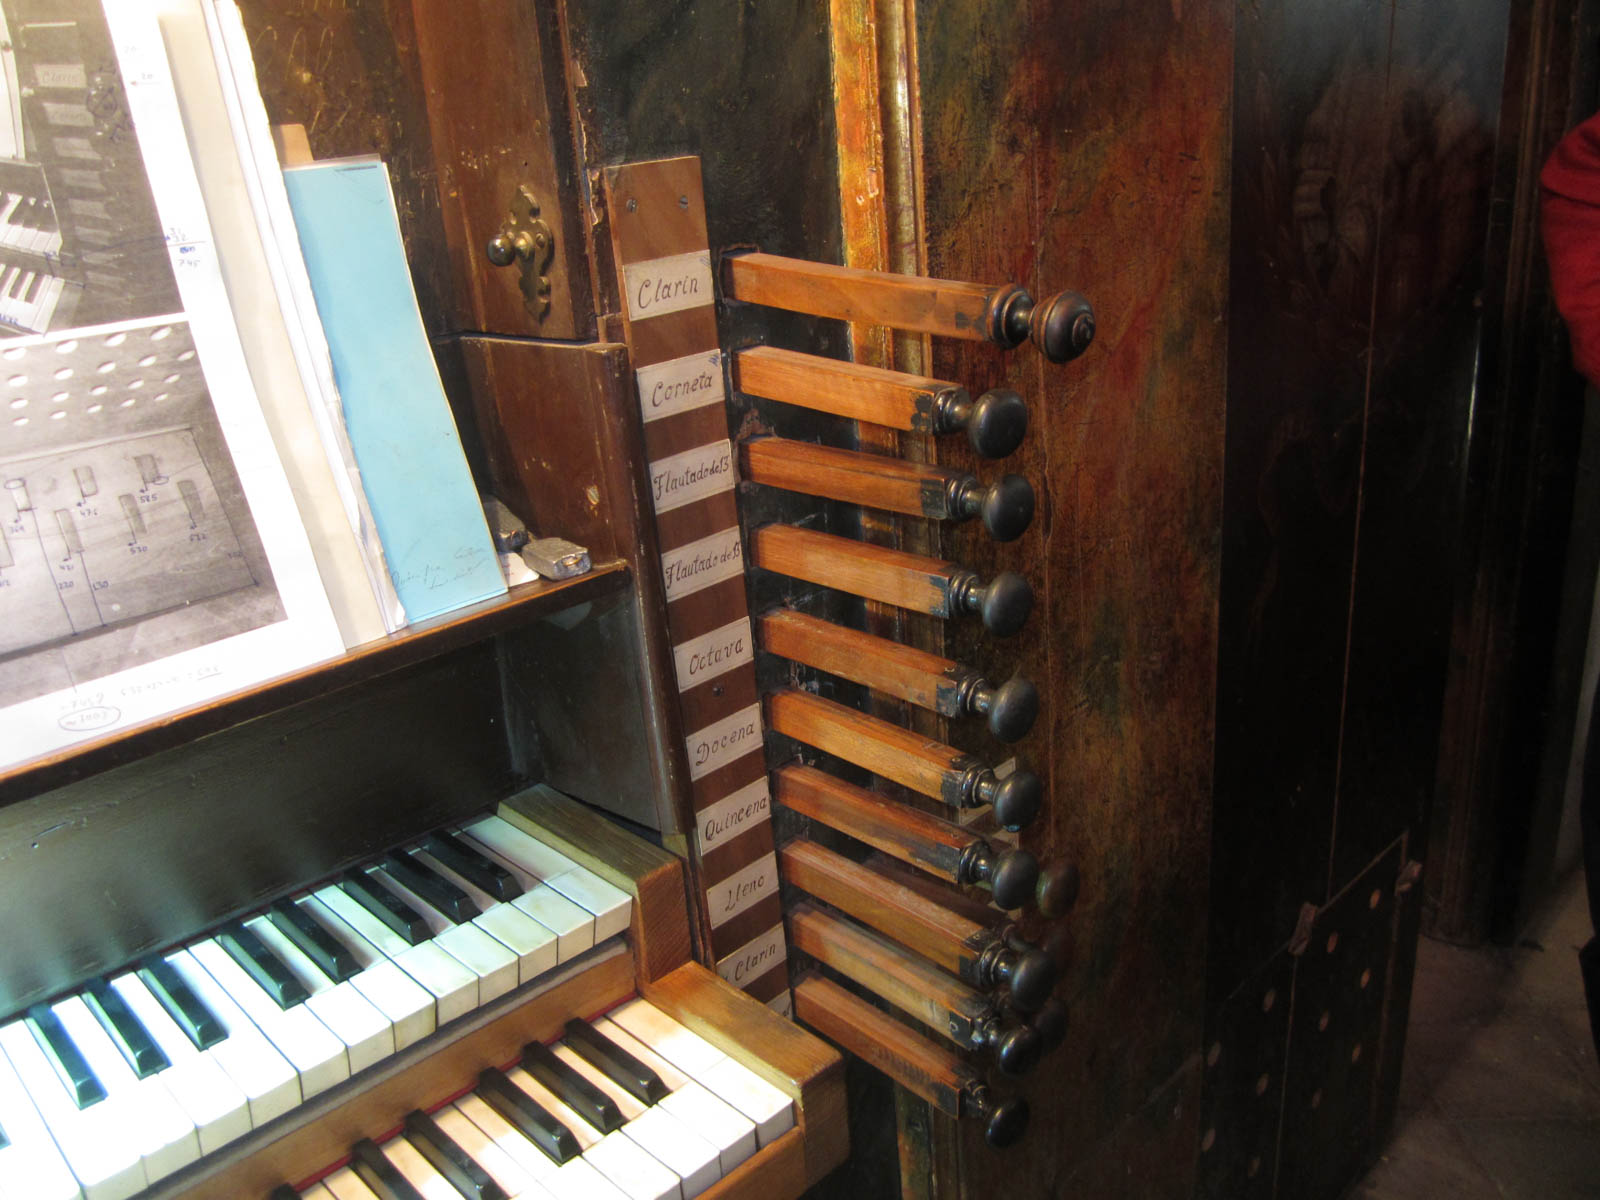
\includegraphics[width=0.4\textwidth]{images/registros} 
			\captionof{figure}{Hilera de registros barrocos.}
		\end{center}
		\columnbreak
		Los registros son las diferentes \textbf{familias de tubos} con el mismo timbre y la misma tesitura. Se pueden abrir o cerrar desde la consola a través de una serie de palancas, de las que se tira para hacer sonar el registro o se empuja para silenciarlo.
	\end{multicols}
	
	\subsection{PCB de control}
	
	\begin{multicols}{2}
		\noindent
		\begin{center}
			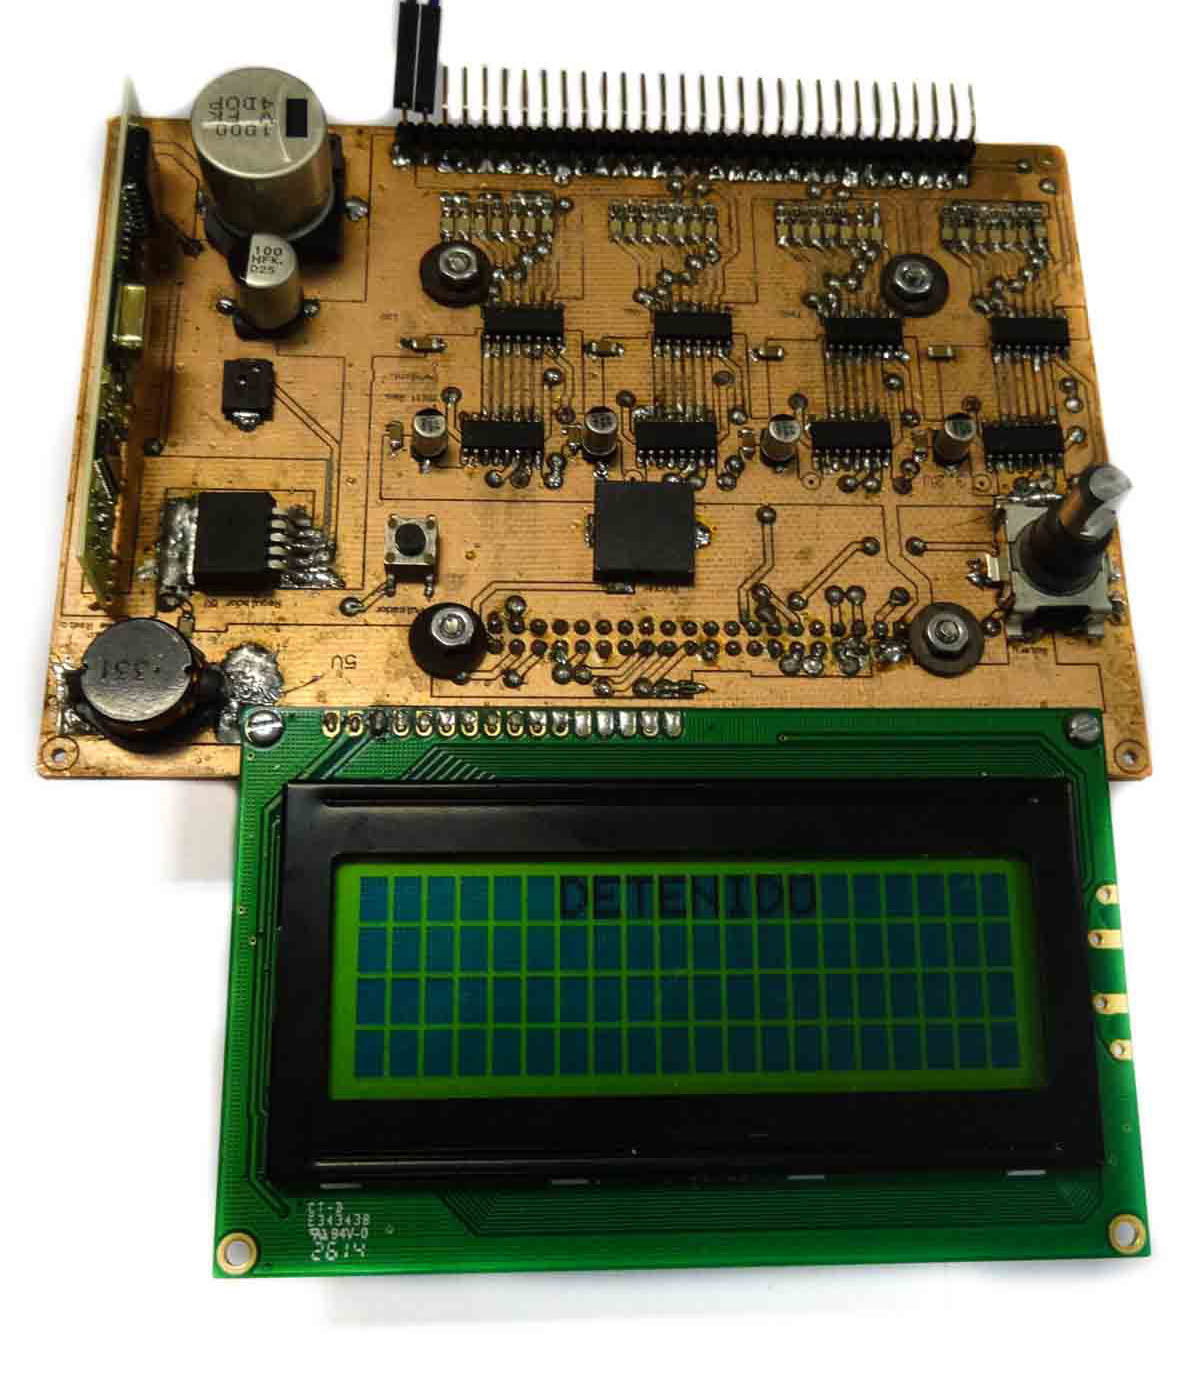
\includegraphics[width=0.4\textwidth]{images/pcb} 
			\captionof{figure}{Prototipo hardware.}
		\end{center}
		\columnbreak
		La placa de circuito impreso es la solución a los requisitos \textit{hardware} aportada por el \textbf{proyecto de Mikel Aguayo Fernández}. 
		
		Incluye una serie de registros de desplazamiento para almacenar el estado del órgano, una interfaz de control local reducido y un medio de control remoto. También alimentará al computador que vamos a utilizar. 
		
		A continuación enumeramos aquellos componentes con los que interactuaremos.		 
	\end{multicols}	
	
	\begin{description}
		\item[Registros de desplazamiento SN74HC595.] Son circuitos lógicos que almacenan una serie de bits. Este modelo, con una capacidad de 8 bits, soporta entrada en serie y salida en paralelo. Usaremos \textbf{cuatro registros} de desplazamiento: uno para cada teclado, otro para el \textit{pedalier} y otro para los registros.
		
		\item[Receptor RF HIRK-433A.] Es un detector de radio con decodificador a interfaz RS-232. Nos da la información del \textbf{número de serie} del mando y qué \textbf{botones} han disparado el evento. 
		
		\item[Pantalla LCD FDCC2004B.] Es un dispositivo genérico de 4 x 20 caracteres. Tiene una pequeña \textbf{memoria} para almacenar el estado e incluye los caracteres ASCII predefinidos.
		
		\item[Codificador rotatorio EC11J.] Es un componente electrónico consistente en un \textbf{botón giratorio y pulsable}. Emite una señal que depende del sentido en que se ha girado el botón.
		
		\item[Zumbador PKLCS1212E4001-R1.] Es un dispositivo piezoeléctrico que produce un sonido agudo continuado. A diferencia de un altavoz, está diseñado para producir \textbf{ondas cuadradas}.
	\end{description}
	
	\subsection{SBC Raspberry Pi}
	
	El \textit{Raspberry Pi} es un \textbf{ordenador} de placa única ---SBC---, más potente que un microcontrolador y con \textbf{sistema operativo} basado en Linux. Se alimenta por USB y se puede controlar con teclado y ratón, o bien desde red mediante SSH.
	
	\begin{multicols}{2}
		\noindent
		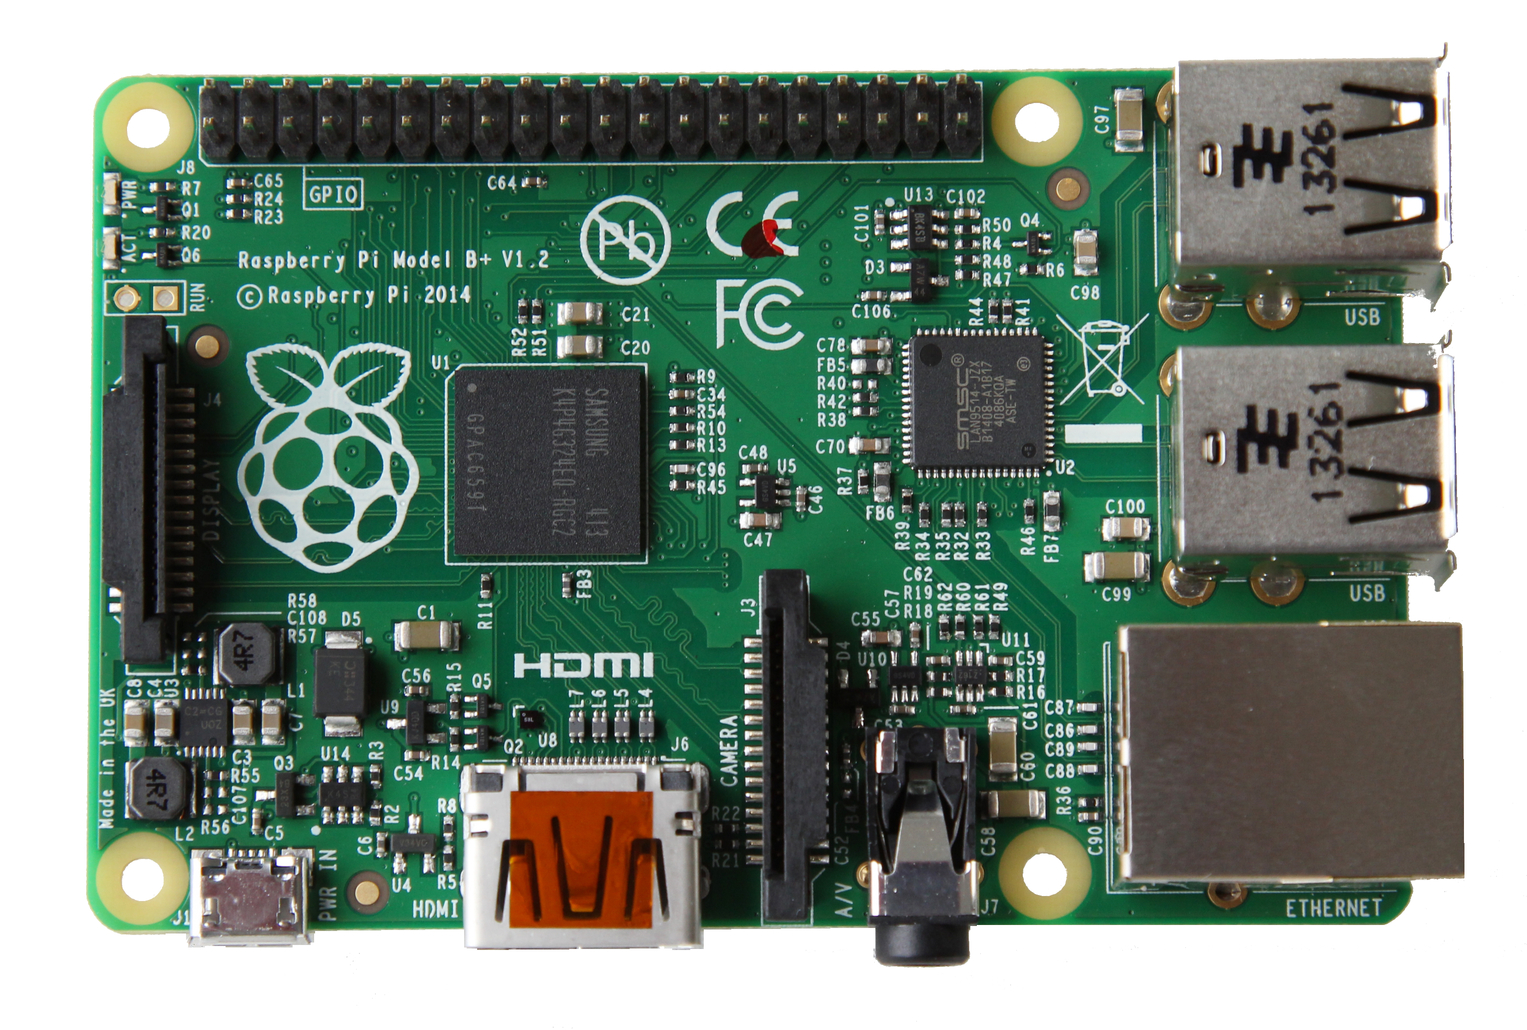
\includegraphics[width=0.5\textwidth]{images/raspberry} 
		\captionof{figure}{Raspberry Pi modelo B.}
		\columnbreak
		El corazón de este computador es un SOC, que integra microprocesador, memoria y periféricos principales.
		
		El modelo escogido, \textit{B+}, posee numerosos pines de entrada y salida de propósito general (GPIO), que utilizaremos para interactuar con la PCB y para ser \textbf{alimentado} por ésta.
	\end{multicols}
	
	 La PCB se conectará al \textit{Raspberry Pi} a través de los conectores GPIO. Todos ellos se utilizarán de forma \textbf{genérica}, excepto el receptor del mando a distancia, que se comunica con la interfaz RS-232 y debe conectarse al \textbf{UART} mediante el pin dedicado a tal periférico.
	 
	 \begin{center}
	 	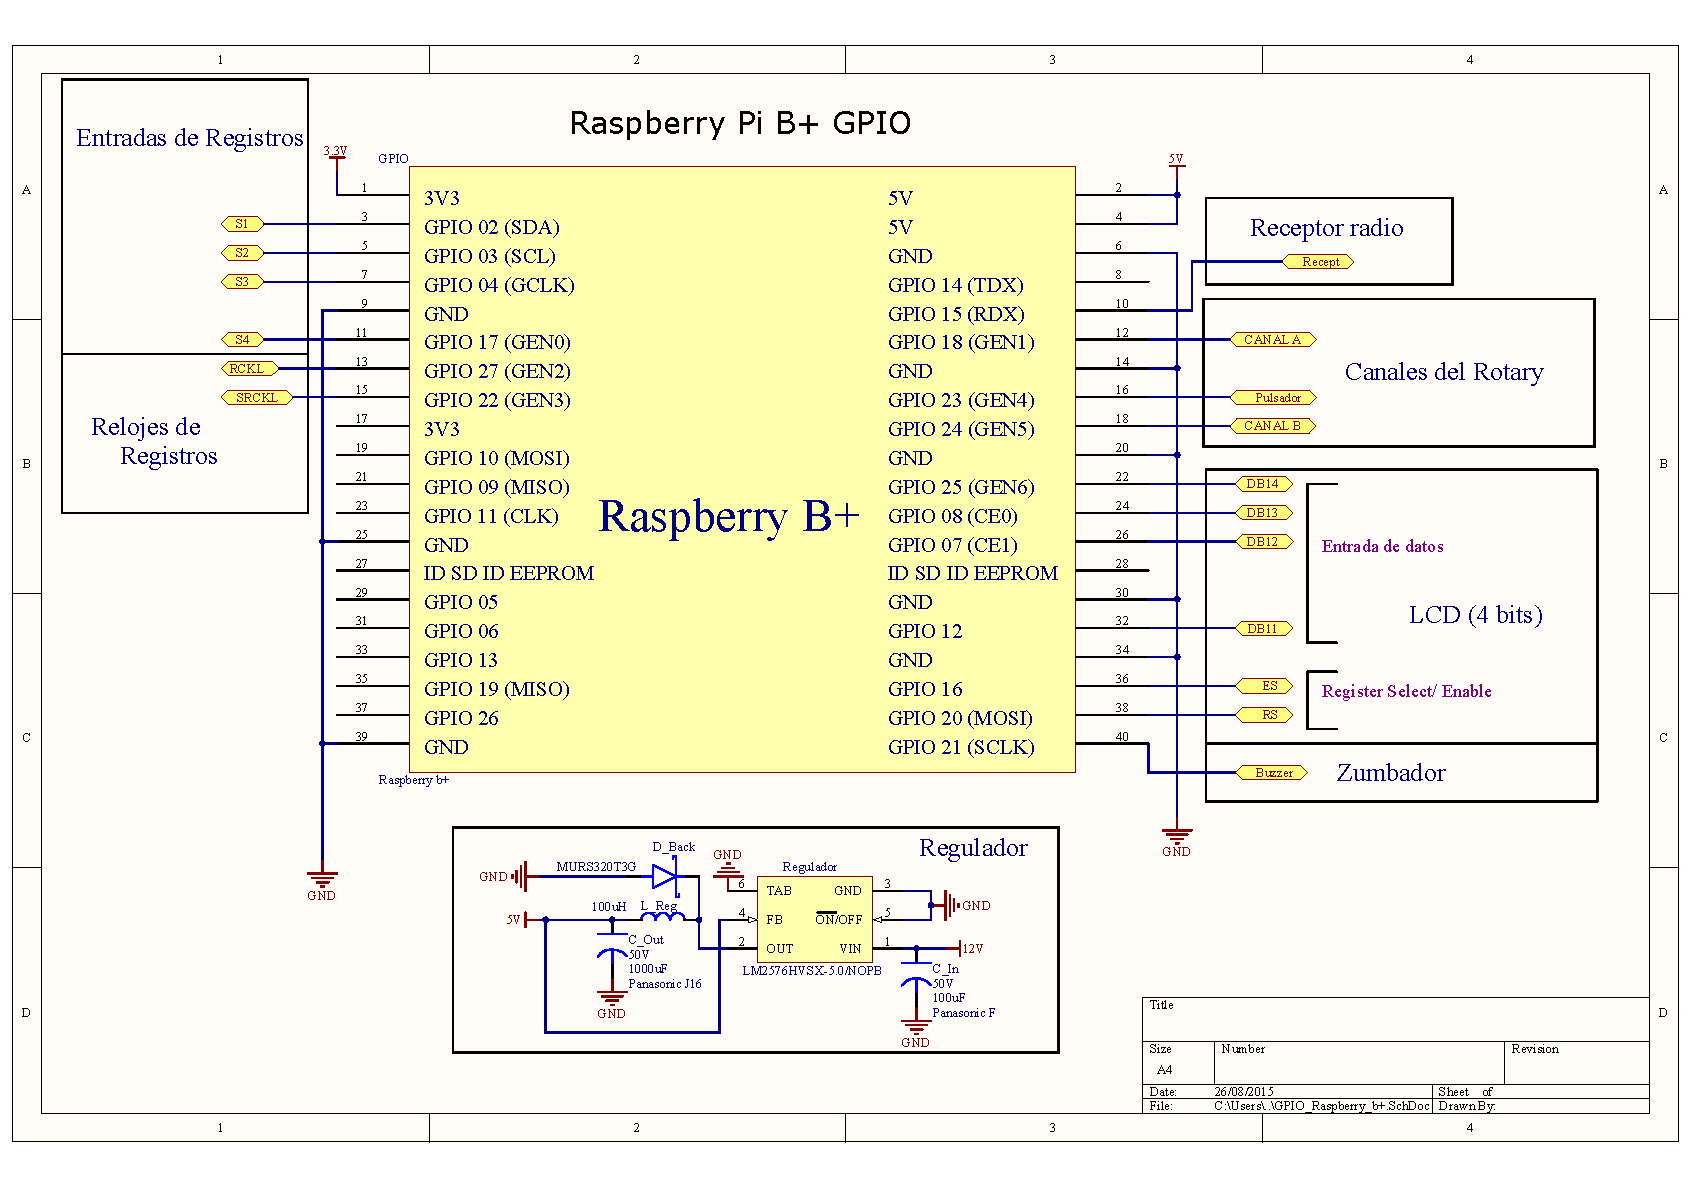
\includegraphics[width=0.75\textwidth]{images/pcb_gpio}
	 	\captionof{figure}{Pines de conexión de la PCB con el Raspberry Pi.}
	 \end{center}
	
	\subsection{Formato de archivo MIDI}
	
	Los datos de entrada a nuestro sistema consisten en archivos MIDI, tal como se menciona en los requisitos. Este tipo de ficheros se presenta como un conjunto de \textbf{bloques} ---\textit{chunks}--- que contienen los eventos clasificados por pistas. Todos los valores numéricos están en formato \textbf{\textit{big-endian}}, detalle a tener en cuenta, ya que tanto la arquitectura x86 como ARM trabajan en \textit{little-endian}.
	
	\begin{description}
		\item[Bloque de cabecera.] Es siempre el \textbf{primero}, empieza por la firma ''MThd'' e incluye el formato, el número de pistas y la división de tiempo.
		
		\item[Bloque de pista.] Consta de una cabecera y de una lista de eventos, que termina con el meta-evento \textit{fin de pista}.
		
		\item[Eventos MIDI.] Cada evento indica el retraso de tiempo respecto al evento anterior, el tipo de evento, el canal y los parámetros correspondientes, tales como la nota o la velocidad de pulsación.
		
		\item[Metaeventos.] Son mensajes de control que extienden la semántica de los eventos. Los más importantes son el \textbf{indicador de \textit{tempo}} y la marca de \textbf{fin de pista}.
		
		\item[Notas.] Se indican numéricamente, en base 0, asignando valores a las notas cromáticas a partir de \textit{Do -1}. Por ejemplo, al \textit{Do central (Do 4)} le corresponde el valor 60.
	\end{description}
	
	\subsection{Interconexión general}
	
	Todos los elementos que hemos descrito conformarán la parte \textit{hardware} del sistema y establecerán una conexión cuyos extremos son el \textbf{computador} \textit{Raspberry Pi} y los \textbf{mecanismos} que interactuarán con la consola del órgano.
	
	\begin{center}
		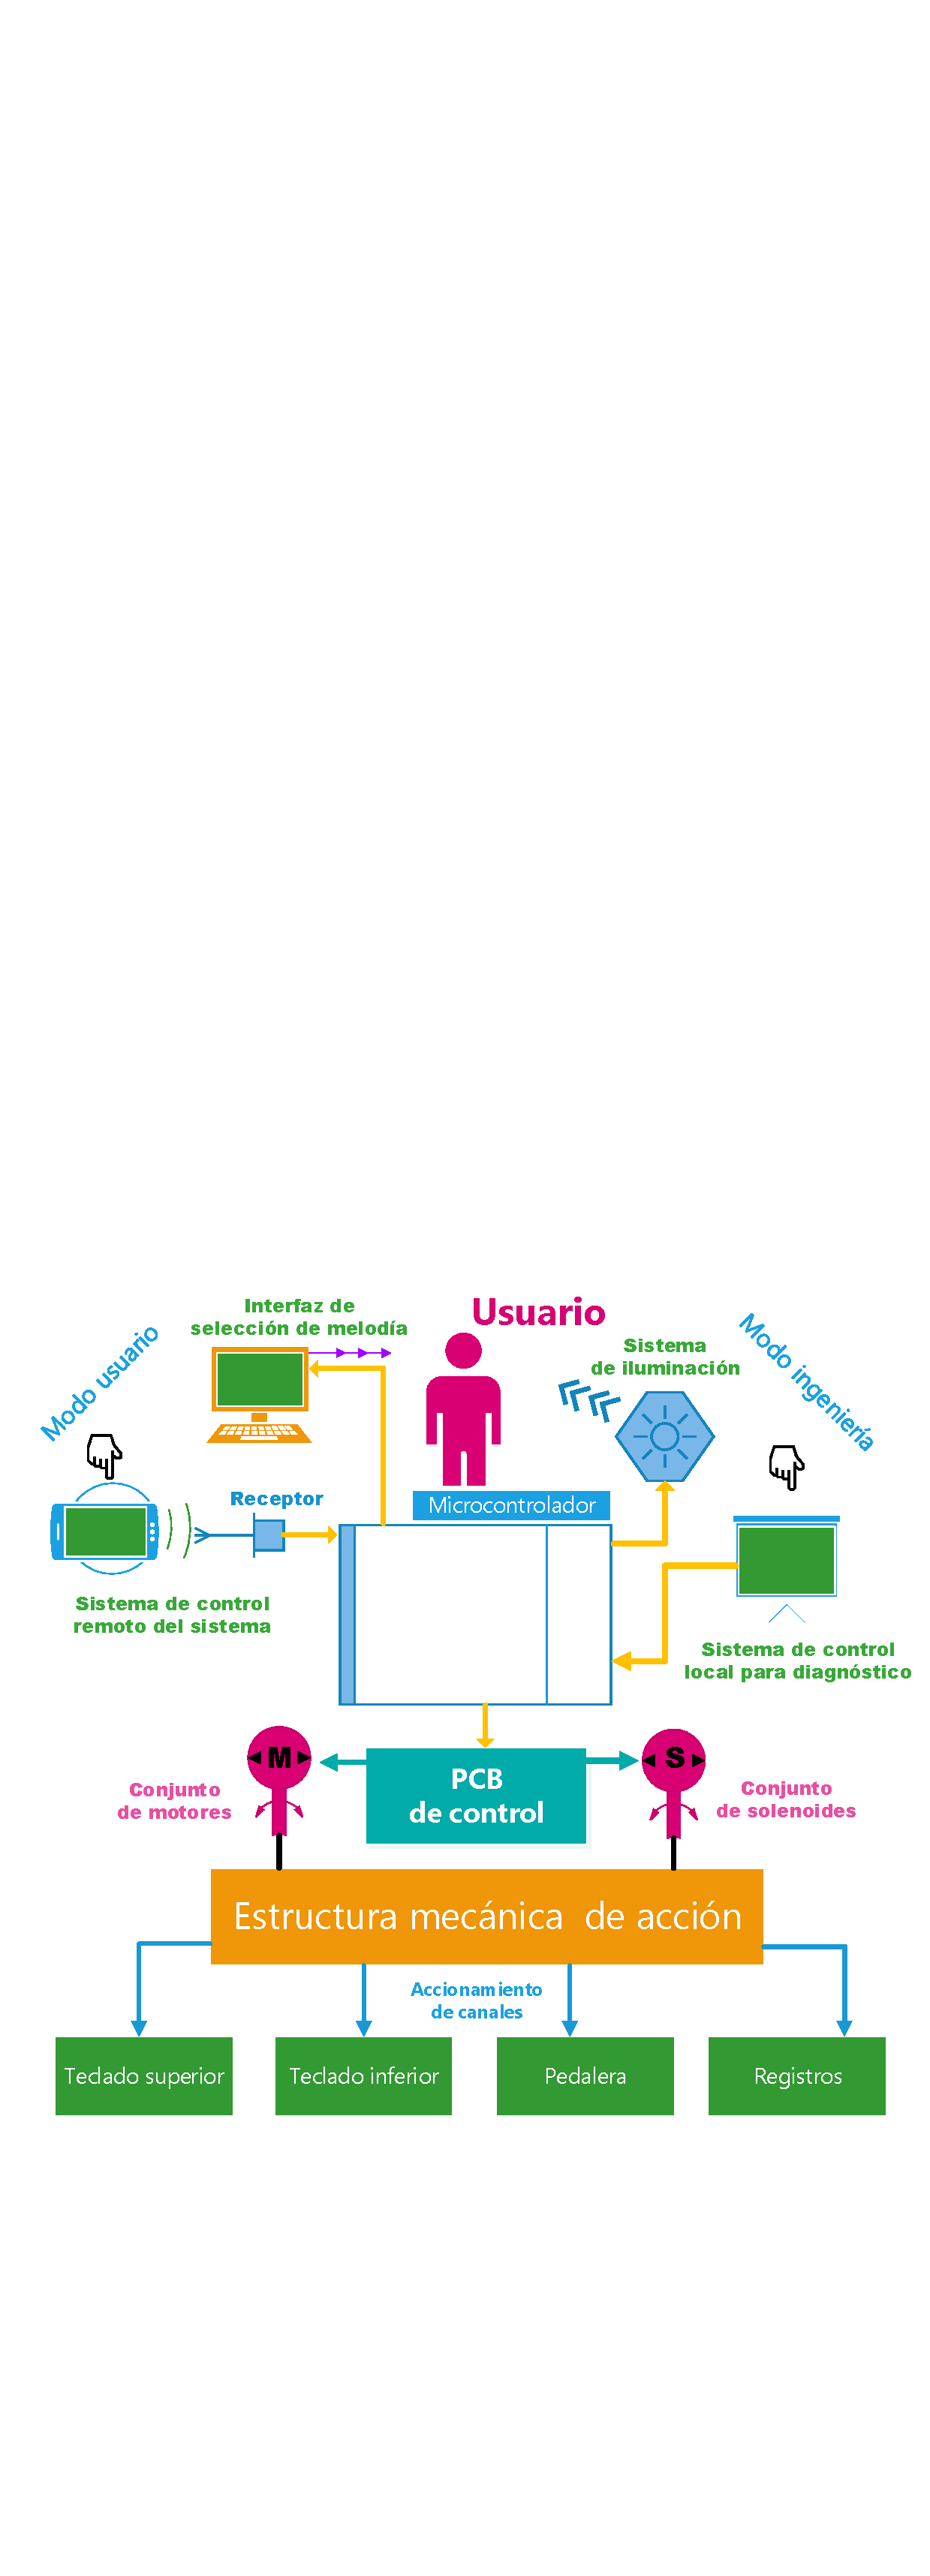
\includegraphics[width=0.75\textwidth]{images/interconexion}
		\captionof{figure}{Conexión lógica entre los elementos hardware.}
	\end{center}
	
	La PCB está conectada mediante la interfaz GPIO. Las conexiones harán funcionar los mecanismos del órgano, pasando por los registros de desplazamiento, que retendrán el estado.
	
	El resto de \textbf{periféricos} de la placa nos serán de utilidad para desarrollar un sistema que cumplirá todos los requisitos contemplados en el proyecto.
	
	% Capítulo 4 ---------------------------------------------------------------
	
	\section{Diseño e implementación}
	
	\subsection{Planteamiento}
	
	\begin{multicols}{2}
		\noindent
		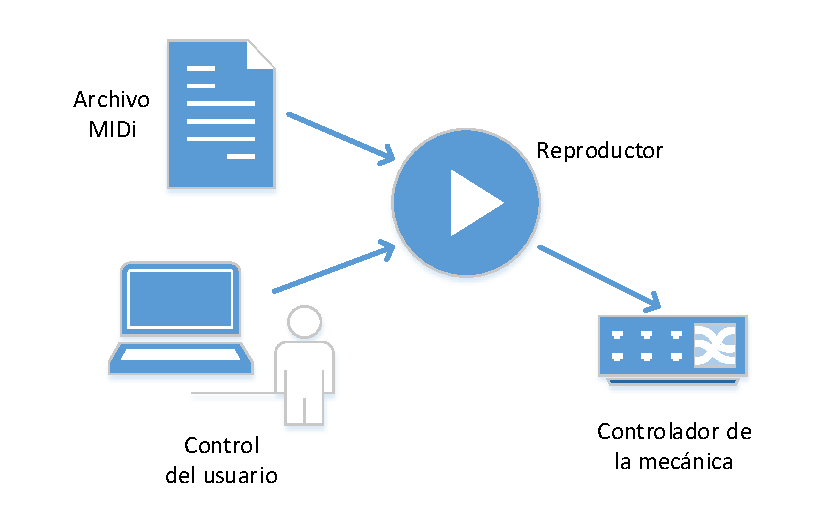
\includegraphics[width=0.5\textwidth]{images/idea} 
		\captionof{figure}{Planteamiento inicial.}
		\columnbreak
		El \textit{software} que tenemos que diseñar consiste en un \textbf{reproductor de archivos MIDI}, que recibe el fichero y lo envía a la PCB a través del GPIO.
		
		Vamos a diseñar el reproductor como un \textbf{demonio} de Linux que, además de gestionar la reproducción de archivos MIDI, proporcionará la interfaz de \textbf{control reducido}, para manejar la mecánica desde la PCB. Además, despachará las órdenes del \textbf{mando a distancia}.
	\end{multicols}
	
	Respecto al de \textbf{control}, se requiere varias formas de acceder al sistema:
	
	\begin{enumerate}
		\item Una \textbf{interfaz \textit{web}} como controlador principal, que cubra todos los casos de uso, y sea fácil de instalar y utilizar. Esta opción permite además que sea multiplataforma.
		
		\item Un mando a distancia, que altere la reproducción.
		
		\item Un control reducido empotrado en la PCB.
	\end{enumerate}
	
	En último lugar, necesitamos \textbf{almacenar información} sobre los archivos MIDI, listas de reproducción y asignaciones del mando en memoria persistente. Una \textbf{base de datos} nos permitiría guardar toda esa información de manera estructurada y coherente, además de ser fácilmente accesible por todos los componentes del sistema.
		
	\begin{center}
		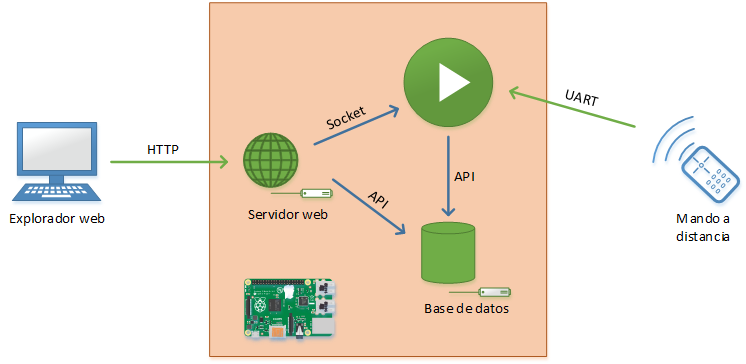
\includegraphics[width=0.75\textwidth]{images/general}
		\captionof{figure}{Diseño general.}
	\end{center}
	
	\subsection{Servicio del reproductor}
	
	\begin{center}
		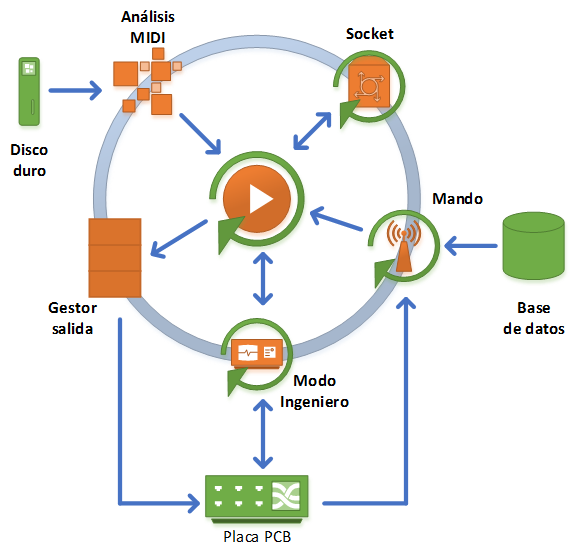
\includegraphics[width=0.75\textwidth]{images/reproductor}
		\captionof{figure}{Diseño interno del reproductor.}
	\end{center}
	
	\subsubsection{Descodificador de MIDI}
	\subsubsection{Planificador}
	\subsubsection{Salida hacia la PCB}
	\subsubsection{Control por socket}
	\subsubsection{Control del mando}
	\subsubsection{Comunicación con la base de datos}
	\subsubsection{Modo ingeniería}
	\subsubsection{Seguridad}
	
	\subsection{Interfaz web}
	
	\subsubsection{Portada}
	\subsubsection{Reproductor}
	\subsubsection{Partituras y listas}
	\subsubsection{Asignación del mando}
	\subsubsection{Energía y multilenguaje}	
	
	\subsection{Base de datos}
	
	\subsection{Aplicaciones auxiliares}
	
	\subsection{Resultado}
	
	% Capítulo 5 ---------------------------------------------------------------
	
	\section{Validación y verificación}
	
	% Capítulo 6 ---------------------------------------------------------------
	
	\section{Conclusión}

\end{document}
